% A 10-minute talk, in plain words, for the supervisor meeting.
% Build (LuaLaTeX: fontspec + babel bidi/onchar): cd docs/talk && lualatex talk.tex && lualatex talk.tex
% Every number is from the E1 / E1b results (docs/e1/, docs/e1b_ros/results.md),
% produced by sim/e1/summarize_e1.py; the "one run" slide is one demo run and says so.
% Citations: papers/<slug>/bibtex.md (verified entries), plus Kaelbling et al. 1998 and
% Stoller et al. 2011. FailSafe, Foresight and Embedding-TL are cited as arXiv preprints
% because no venue is verified for them.
\documentclass[14pt, aspectratio=169]{beamer}
\usetheme{Madrid}

% --- UNIVERSAL PREAMBLE BLOCK ---
\usepackage{fontspec}
\usepackage[english, bidi=basic, provide=*]{babel}
\babelprovide[onchar=ids fonts]{english} % "import" dropped: english is already loaded above, and babel v24.1 (Ubuntu 24.04 TeX Live) would define \englishdate twice

% Set default/Latin font to Sans Serif in the main (rm) and sans (sf) slot for Beamer
\babelfont{rm}{Noto Sans}
\babelfont{sf}{Noto Sans}

\usepackage{tikz}
\usetikzlibrary{shapes, arrows.meta, fit, positioning, calc}
\usepackage{amsmath}

% --- BEAMER CONFIGURATION ---
% Remove the navigation option bar from the bottom left corner
\setbeamertemplate{navigation symbols}{}
\setbeamertemplate{itemize items}[circle]

% --- THIS TALK ---
\usepackage{array}
\definecolor{acc}{HTML}{1F5FAE}
\definecolor{bad}{HTML}{B5503C}
\definecolor{mut}{HTML}{5B6472}
\definecolor{soft}{HTML}{EEF1F5}
\newcommand{\key}[1]{\textbf{\color{acc}#1}}
\newcommand{\pic}[1]{\par\vspace{0.1cm}{\scriptsize\color{mut}#1\par}}
\newcommand{\cit}[1]{{\color{mut}[#1]}}

\title[Skill progress monitoring]{Skill progress monitoring}
\subtitle{Catching robot failures while they happen}
\author[P. N. Aburmad]{Pinhas Nehoray Aburmad}
\institute[BGU]{Ben-Gurion University of the Negev\\ Supervisor: Prof.\ Ronen Brafman}
\date{}
\titlegraphic{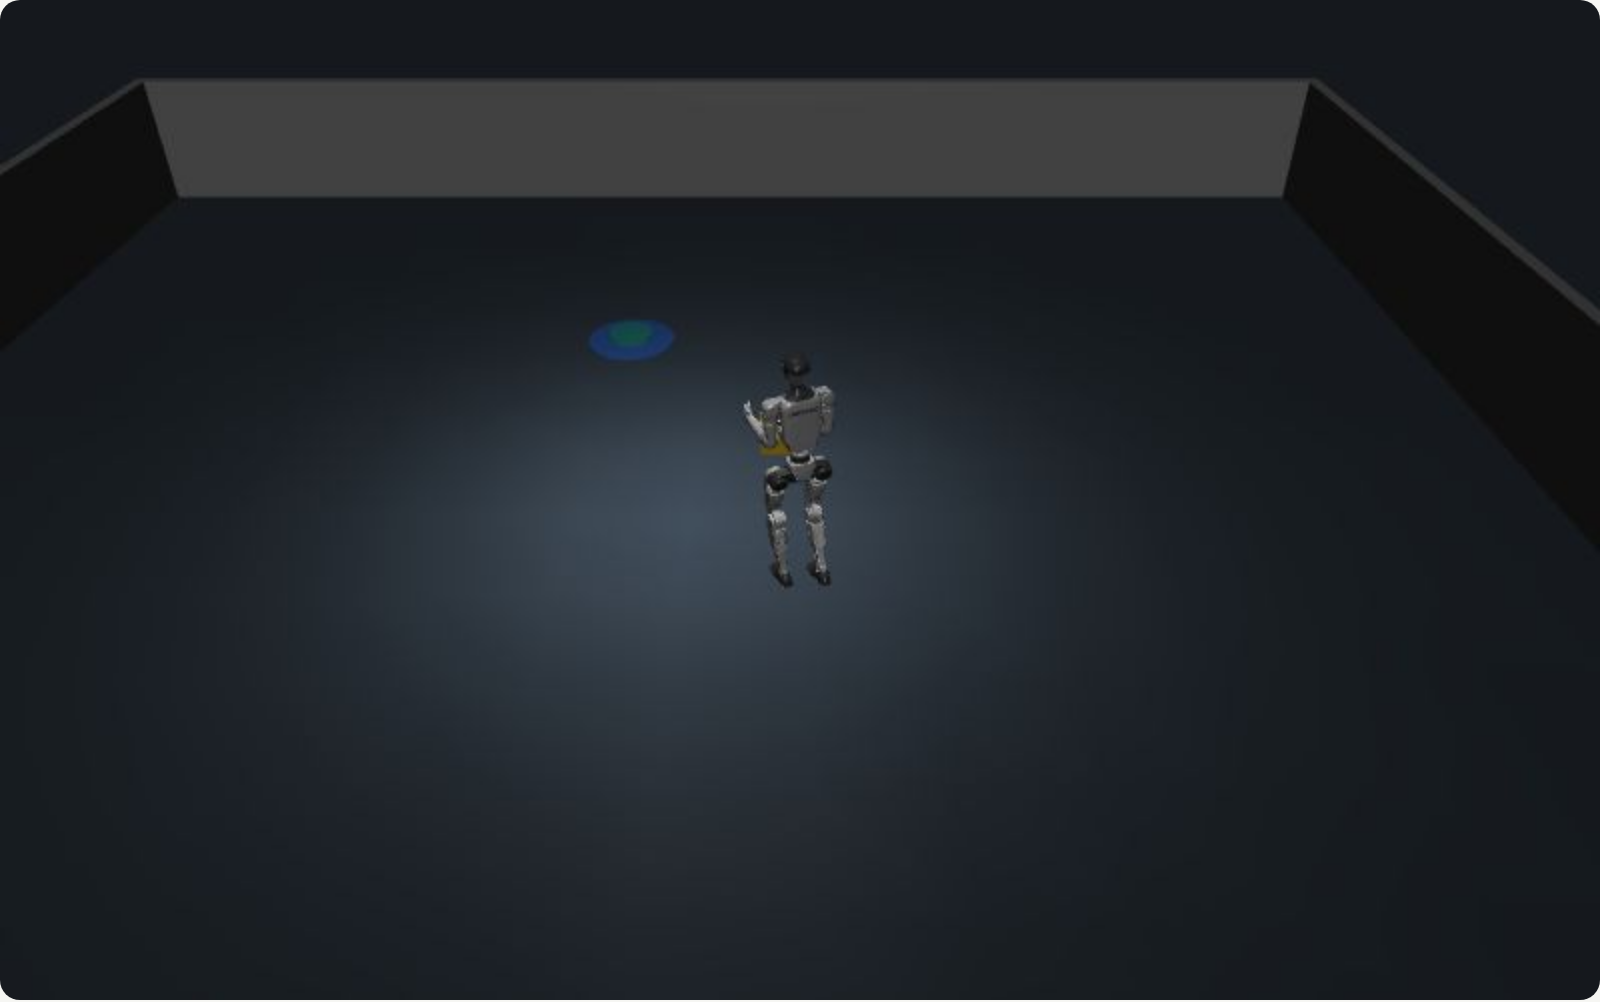
\includegraphics[height=1.55cm]{figures/robot_title.png}}

\begin{document}

% --- TITLE SLIDE ---
\begin{frame}
    \titlepage
\end{frame}

% --- THE PROBLEM ---
\begin{frame}{The problem}
    \begin{columns}[c]
        \begin{column}{0.50\textwidth}
            \begin{itemize}
                \item Robots often fail \textbf{in the middle} of a task.
                \item They often \textbf{do not notice}.
                \item They report ``done'' anyway.
                \item \key{Goal:} notice the failure \key{the moment it happens}.
            \end{itemize}
        \end{column}
        \begin{column}{0.48\textwidth}
            \centering
            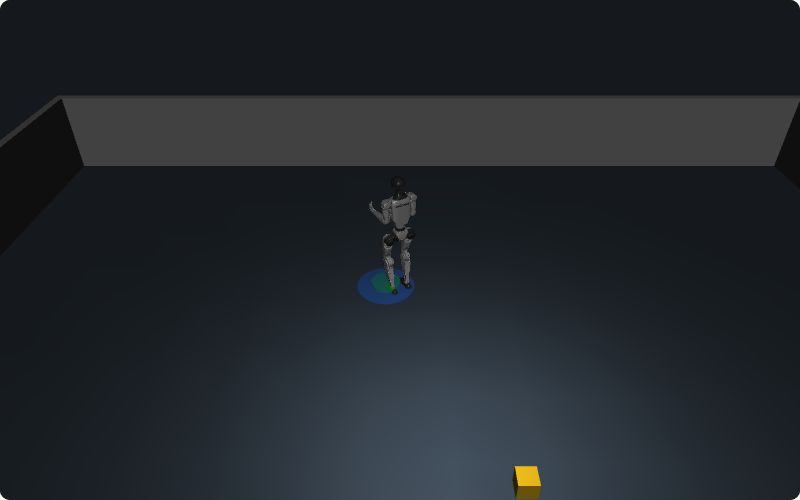
\includegraphics[width=\linewidth]{figures/robot_false_success.png}
            \pic{The robot says ``done'' at the drop-off (blue). The box (yellow) is still on the floor.}
        \end{column}
    \end{columns}
\end{frame}

% --- RELATED WORK ---
\begin{frame}{Related work}
    \footnotesize
    \renewcommand{\arraystretch}{1.12}
    \begin{tabular}{@{}>{\raggedright\arraybackslash}p{0.32\linewidth} >{\raggedright\arraybackslash}p{0.28\linewidth} >{\raggedright\arraybackslash}p{0.34\linewidth}@{}}
        \textbf{Work} & \textbf{What it does} & \textbf{\color{bad}What is missing} \\ \hline
        Runtime verification of LTL \cit{Bauer 2011} & checks rules on a running system & no task stages: ``eventually'' says nothing until the end \\
        Robot monitors for ROS \cit{Ferrando 2020; Yamaguchi 2024} & check rules on robot messages & rules written by hand; no task progress \\
        Monitoring with a hidden state \cit{Stoller 2011} & guesses the hidden state with a probability model & needs that model; no task stages \\
        English $\to$ logic \cit{Liu 2023; Cosler 2023; Chen 2023} & turn words into LTL rules & used to plan, not to watch a running task \\
        Learned failure detectors \cit{Lin 2025; Zhang 2026; Kapoor 2026} & learn failures from camera data & need training data; hard to say why it fired \\ \hline
    \end{tabular}
    \vspace{0.25cm}

    \normalsize
    \key{Our gap:} rules made from plain words \textbf{+} task stages \textbf{+} only the robot's own sensors.
\end{frame}

% --- BACKGROUND ---
\begin{frame}{Background: what is a monitor?}
    \begin{columns}[c]
        \begin{column}{0.56\textwidth}
            \begin{itemize}
                \item A program that \textbf{watches} the robot's messages.
                \item It checks \textbf{rules over time}, written in \key{LTL} (a logic of time).
                \item Example: ``\emph{always} stay upright''.
                \item Each rule becomes a small \textbf{state machine}.
                \item Problem: ``\emph{eventually} deliver'' \textbf{never fails early}.
            \end{itemize}
        \end{column}
        \begin{column}{0.42\textwidth}
            \centering
            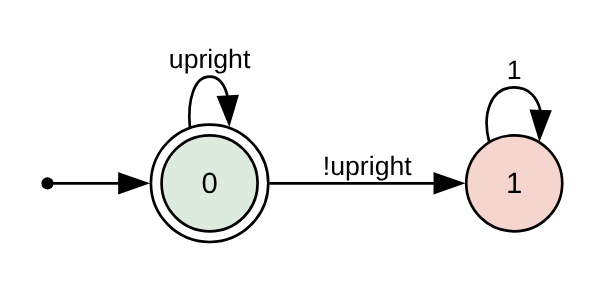
\includegraphics[width=\linewidth]{figures/aut_fell_over.png}
            \pic{``Always upright'' as a state machine. One fall moves it to state 1 (red), forever.}
        \end{column}
    \end{columns}
\end{frame}

% --- OUR IDEA ---
\begin{frame}{Our idea: the stages of the task}
    \textbf{Each stage has its own rules and its own time limit.}
    \vspace{0.3cm}

    \centering
    \resizebox{0.95\linewidth}{!}{
    \begin{tikzpicture}[
        st/.style={draw=mut, rounded corners=4pt, fill=soft, minimum width=2.4cm, minimum height=1.3cm, align=center},
        hot/.style={st, draw=acc, line width=1.4pt, fill=acc!10},
        arr/.style={-{Stealth[length=2.5mm]}, thick, mut},
        flt/.style={-{Stealth[length=2.2mm]}, dashed, draw=bad}]
        \node[st] (w) {\textbf{Walk to box}\\ $\le 45$ s};
        \node[st, right=0.5cm of w] (g) {\textbf{Grasp}\\ $\le 10$ s};
        \node[hot, right=0.5cm of g] (c) {\textbf{Carry}\\ $\le 60$ s\\ \color{acc}must hold box};
        \node[st, right=0.5cm of c] (p) {\textbf{Place}\\ $\le 10$ s};
        \node[st, right=0.5cm of p, fill=green!8] (d) {\textbf{Done}};
        \node[st, below=0.8cm of c, fill=bad!12, draw=bad, minimum width=9cm] (f) {\color{bad}\textbf{Failure:} a rule broke, too slow, or stuck};
        \draw[arr] (w) -- (g); \draw[arr] (g) -- (c); \draw[arr] (c) -- (p); \draw[arr] (p) -- (d);
        \foreach \n in {w, g, c, p} \draw[flt] (\n.south) -- (f.north -| \n.south);
    \end{tikzpicture}
    }
    \vspace{0.2cm}

    \raggedright
    While carrying, the robot \textbf{must hold the box}. A drop is caught \key{at once}.
\end{frame}

% --- THE MATHEMATICAL MODEL ---
\begin{frame}{The mathematical model: a POMDP}
    \begin{columns}[c]
        \begin{column}{0.58\textwidth}
            \small
            \begin{itemize}
                \item \textbf{Hidden} $s$: what really happens (stage, box held?).
                \item \textbf{Seen} $o$: the robot's messages.
                \item \textbf{Belief} $b$: our best guess of $s$.
                \item \textbf{Action} $a$: continue, stop, or re-plan.
            \end{itemize}
            \vspace{-0.1cm}
            \[
                b'(s') \;\propto\; \underbrace{Z(o \mid s')}_{\text{does $o$ fit $s'$?}} \sum_{s} \underbrace{T(s' \mid s, a)}_{\text{how $s$ changes}}\, b(s)
            \]
            \vspace{-0.2cm}

            \key{Today:} the guess is one point (stage + rule states); the update is one rule step.
        \end{column}
        \begin{column}{0.40\textwidth}
            \centering
            \resizebox{\linewidth}{!}{
            \begin{tikzpicture}[
                bx/.style={draw=mut, rounded corners=4pt, fill=soft, minimum height=1.2cm, text width=7.2cm, align=center},
                arr/.style={-{Stealth[length=2.5mm]}, thick, mut}]
                \node[bx, fill=bad!8, draw=bad] (s) {\textbf{Hidden $s$}\\ true stage, box held?};
                \node[bx, below=0.8cm of s] (o) {\textbf{Seen $o$}\\ noisy robot messages};
                \node[bx, below=0.8cm of o, draw=acc, line width=1.4pt, fill=acc!10] (b) {\textbf{Belief $b$}\\ stage + rule states};
                \node[bx, below=0.8cm of b] (a) {\textbf{Action $a$}\\ continue / stop / re-plan};
                \draw[arr] (s) -- node[right, color=mut]{$Z$} (o);
                \draw[arr] (o) -- node[right, color=mut]{update} (b);
                \draw[arr] (b) -- node[right, color=mut]{decide} (a);
                \draw[arr] (a.west) -- ++(-0.7, 0) |- node[pos=0.25, left, color=mut]{$T$} (s.west);
            \end{tikzpicture}
            }
            \pic{POMDP \cit{Kaelbling 1998}. Why stages help: ``not holding'' is fine while walking, a failure while carrying.}
        \end{column}
    \end{columns}
\end{frame}

% --- METHOD ---
\begin{frame}{Method: how the monitor is built and run}
    \centering
    \resizebox{\linewidth}{!}{
    \begin{tikzpicture}[
        bx/.style={draw=mut, rounded corners=4pt, fill=soft, minimum height=1.6cm, text width=3.8cm, align=center},
        arr/.style={-{Stealth[length=2.5mm]}, thick, mut}]
        \node[bx] (t) {\textbf{Task in words}\\ ``walk to the box, pick it up''};
        \node[bx, right=0.5cm of t] (l) {\textbf{An LLM}\\ writes the stages and rules};
        \node[bx, right=0.5cm of l] (s) {\textbf{Spot} (a tool)\\ rules $\to$ state machines};
        \node[bx, right=0.5cm of s, draw=acc, line width=1.4pt, fill=acc!10] (m) {\textbf{Monitor}\\ checks once a second};
        \node[bx, right=0.5cm of m, fill=bad!10, draw=bad] (a) {\textbf{Alarm}\\ report, stop or re-plan};
        \node[bx, below=0.9cm of m, text width=8cm] (r) {\textbf{Robot messages} (ROS~2)\\ position, laser, box position};
        \draw[arr] (t) -- (l); \draw[arr] (l) -- (s); \draw[arr] (s) -- (m); \draw[arr] (m) -- (a); \draw[arr] (r) -- (m);
    \end{tikzpicture}
    }
    \vspace{0.1cm}

    \raggedright
    \begin{itemize}
        \item The rules are written \textbf{automatically}, from the task in words.
        \item The monitor uses \textbf{only sensors}. It never asks the planner.
    \end{itemize}
\end{frame}

% --- TEST BED ---
\begin{frame}{Test bed: a humanoid robot in a simulator}
    \begin{itemize}
        \item Unitree \textbf{G1} robot in the \textbf{MuJoCo} physics simulator.
        \item We \key{cause failures on purpose}: push, stall, drop, failed grasp.
        \item We compare the monitor \key{with stages} and \key{without}.
    \end{itemize}
    \vspace{0.1cm}
    \centering
    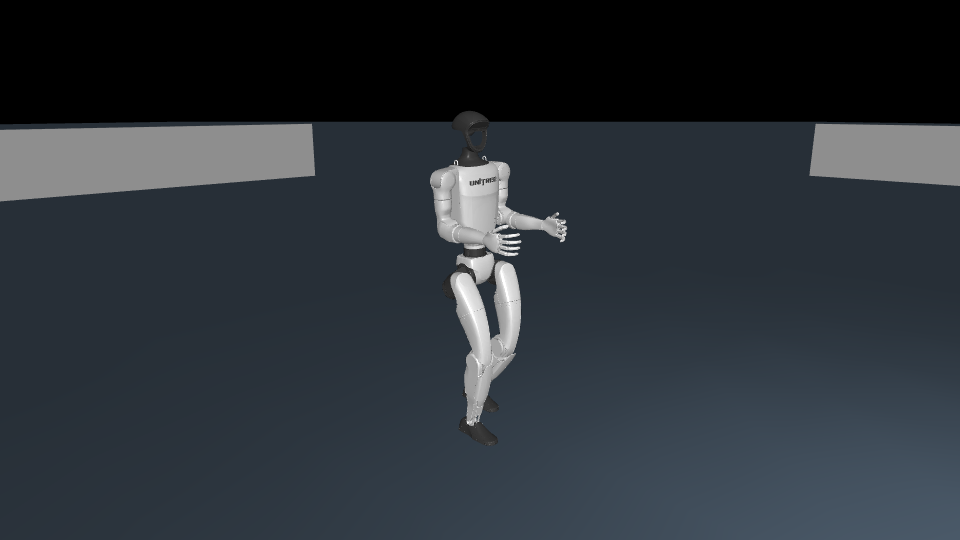
\includegraphics[width=0.3\linewidth]{figures/frame_push_1_walking.png}\hfill
    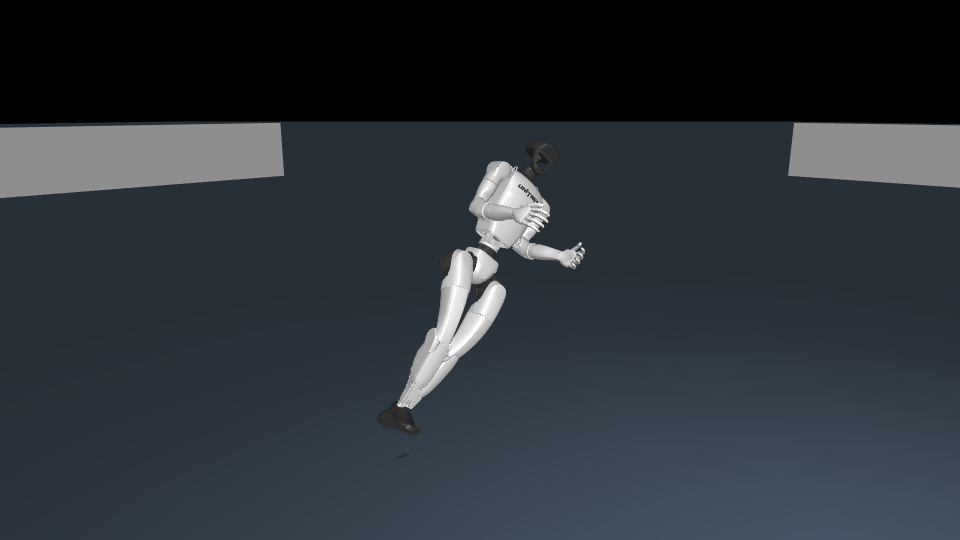
\includegraphics[width=0.3\linewidth]{figures/frame_push_2_pushed.png}\hfill
    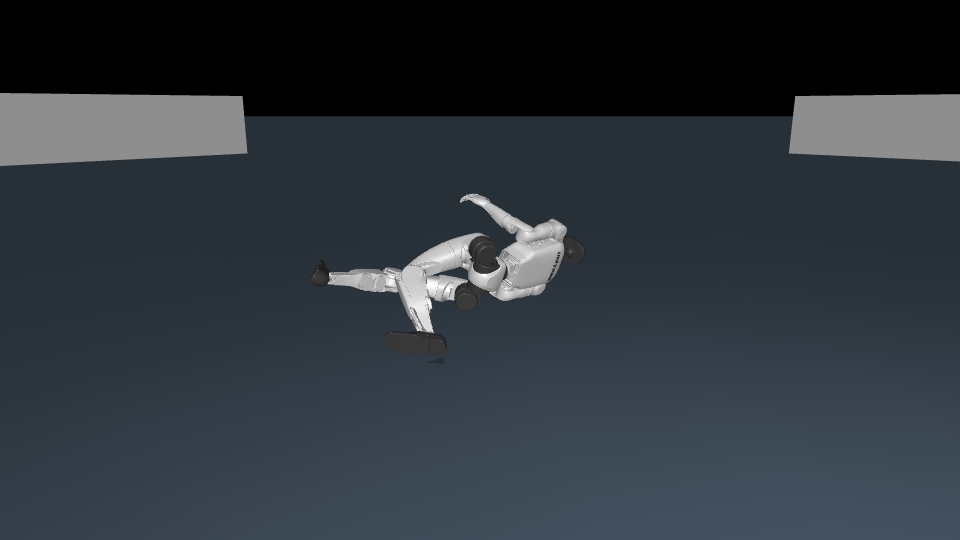
\includegraphics[width=0.3\linewidth]{figures/frame_push_3_down.png}
    \pic{Walking $\rightarrow$ pushed $\rightarrow$ fallen. The simulator knows the truth; the monitor does not.}
\end{frame}

% --- EXPERIMENT 1 ---
\begin{frame}{Experiment 1: a short walk (1800 runs)}
    \begin{columns}[c]
        \begin{column}{0.44\textwidth}
            \begin{itemize}
                \item Stages helped \textbf{little} here: 15 vs.\ 14 of 15 stalls caught.
                \item What mattered: measure progress \key{from the robot's sensors}.
                \item Without that: only \textbf{1 of 15} caught.
            \end{itemize}
        \end{column}
        \begin{column}{0.54\textwidth}
            \centering
            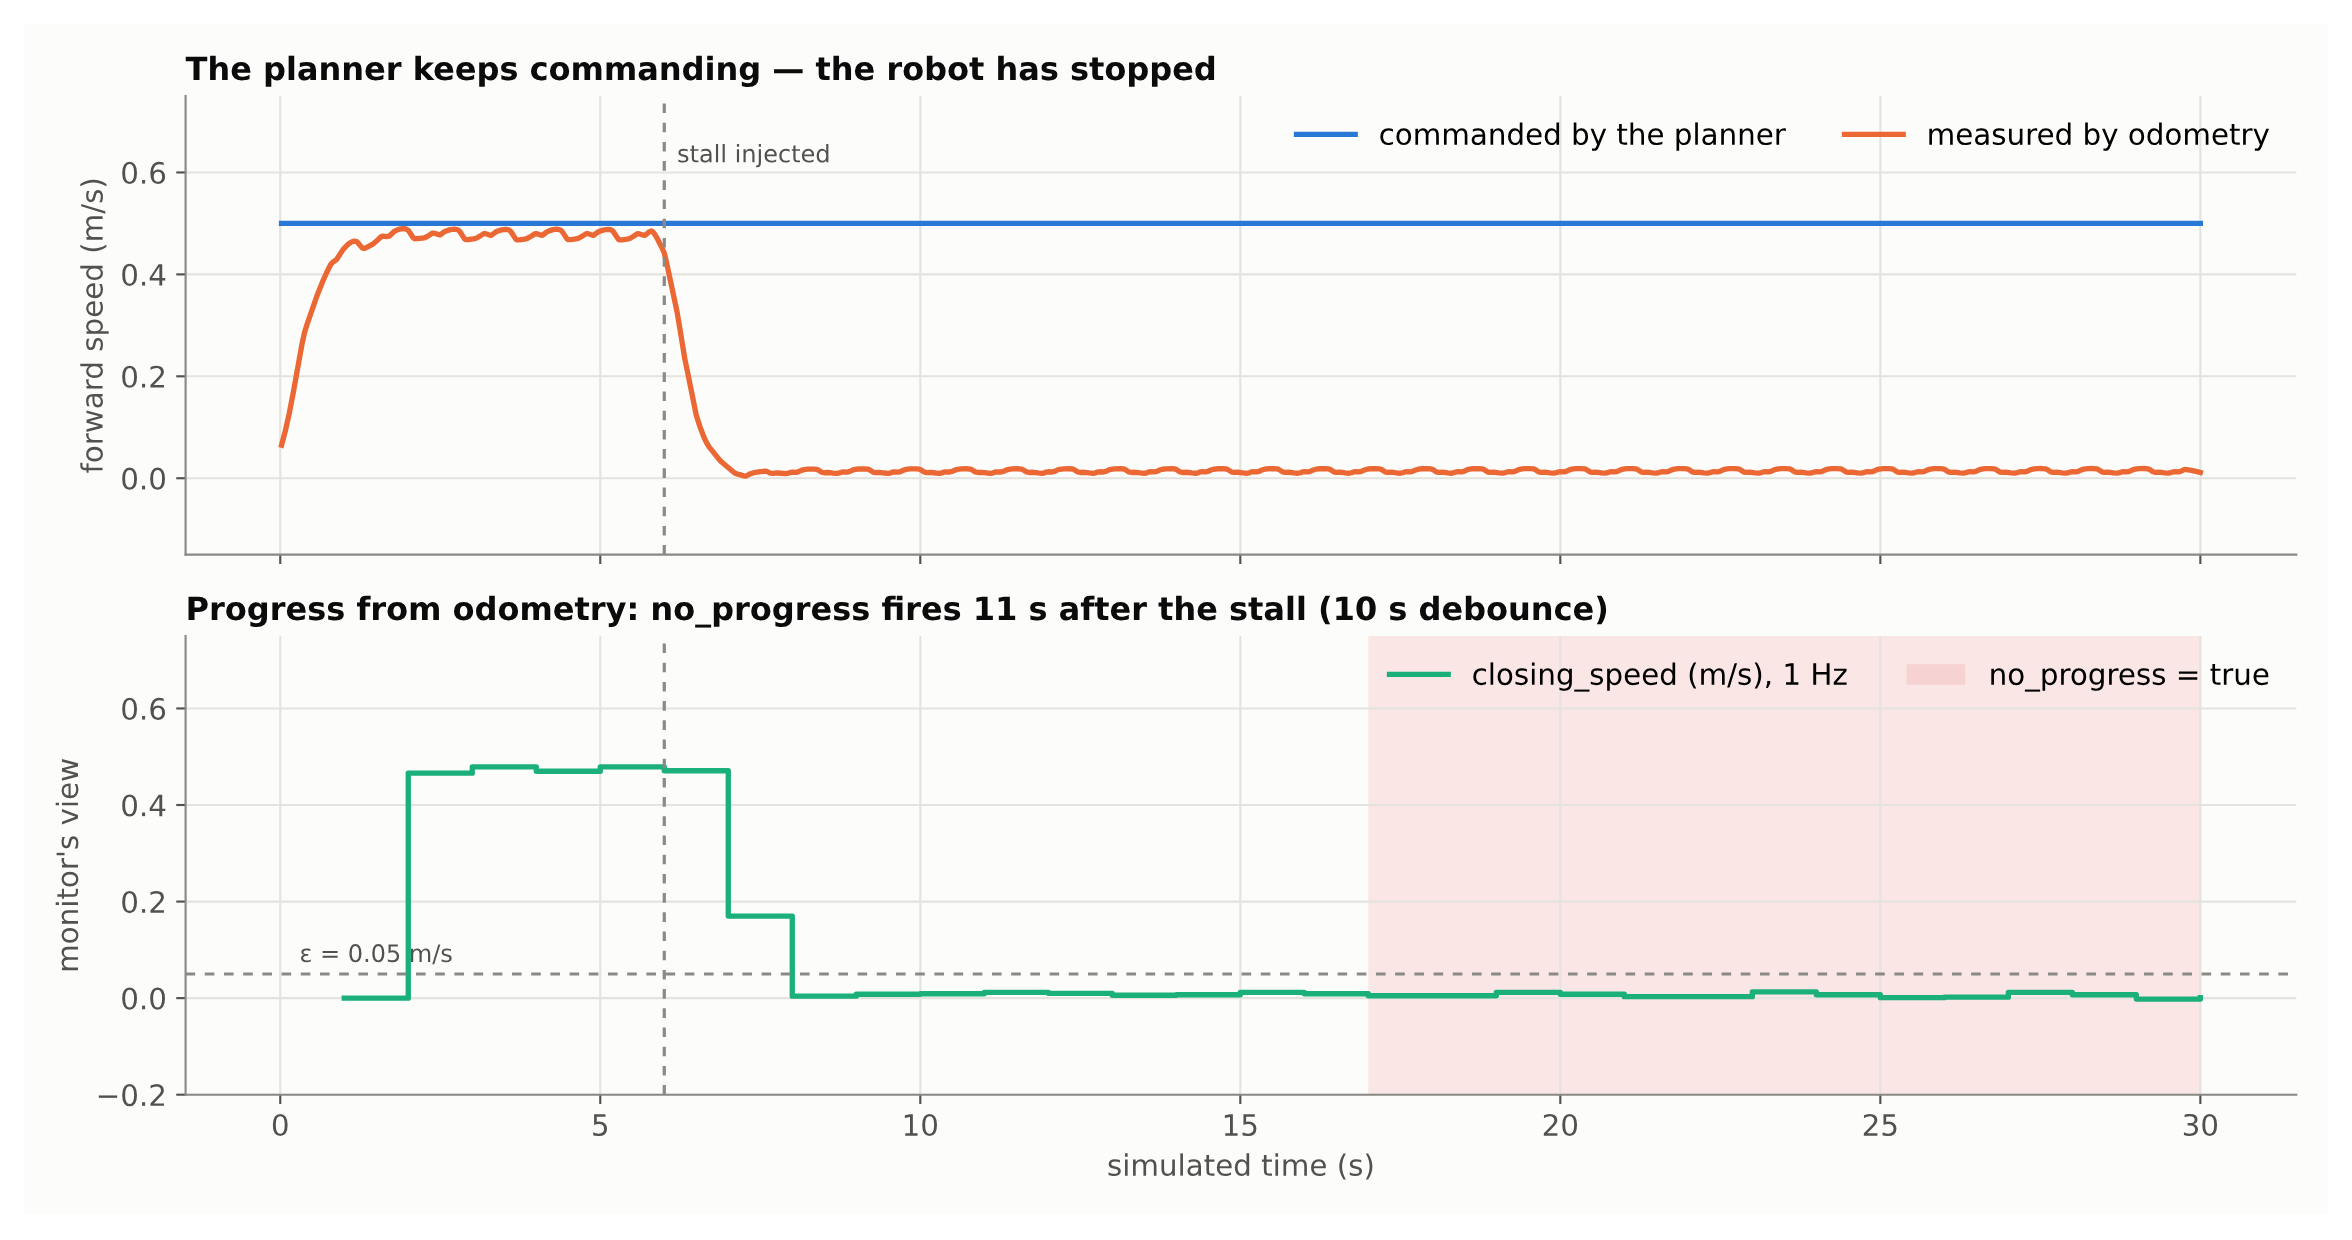
\includegraphics[width=\linewidth]{figures/stall.png}
            \pic{The planner still says ``go''. The robot has stopped. The monitor sees no progress.}
        \end{column}
    \end{columns}
\end{frame}

% --- EXPERIMENT 2 ---
\begin{frame}{Experiment 2: fetch and deliver (3360 runs)}
    \begin{columns}[c]
        \begin{column}{0.42\textwidth}
            \begin{itemize}
                \item Four stages.
                \item Box dropped: caught after \key{1~s} with stages, 14~s without.
                \item Grasp failed: \key{4~s} vs.\ 19~s.
                \item Earlier in \textbf{all 20} runs.
            \end{itemize}
        \end{column}
        \begin{column}{0.56\textwidth}
            \centering
            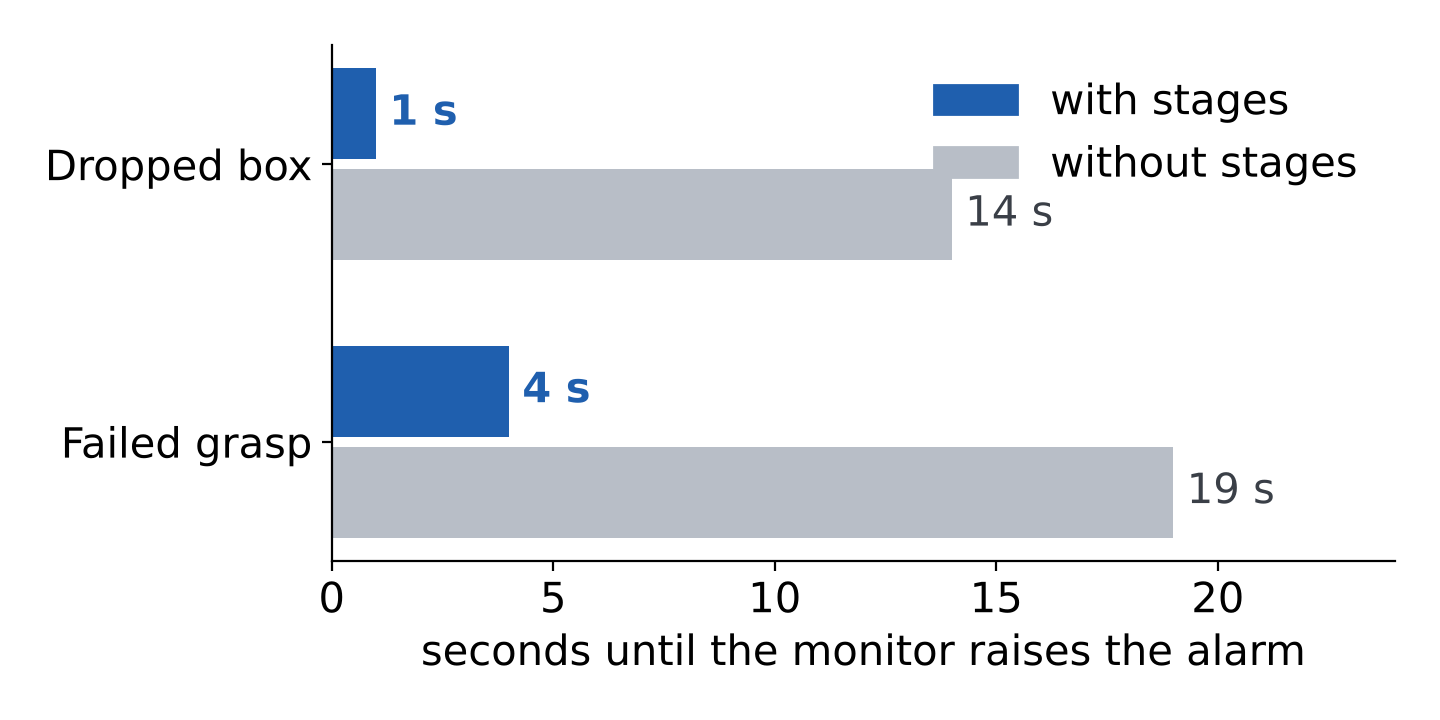
\includegraphics[width=\linewidth]{figures/chart_latency.png}
            \pic{Middle value (median) of 20 runs for each failure.}
        \end{column}
    \end{columns}
\end{frame}

% --- ONE RUN ---
\begin{frame}{One run, second by second}
    \begin{columns}[c]
        \begin{column}{0.40\textwidth}
            \begin{itemize}
                \item \textbf{21.6~s:} the box drops.
                \item \textbf{\color{bad}22~s:} the Carry rule breaks. Alarm.
                \item The plain LTL rule still waits: ``maybe later''.
            \end{itemize}
            \textbf{The stage caught it.}
        \end{column}
        \begin{column}{0.58\textwidth}
            \centering
            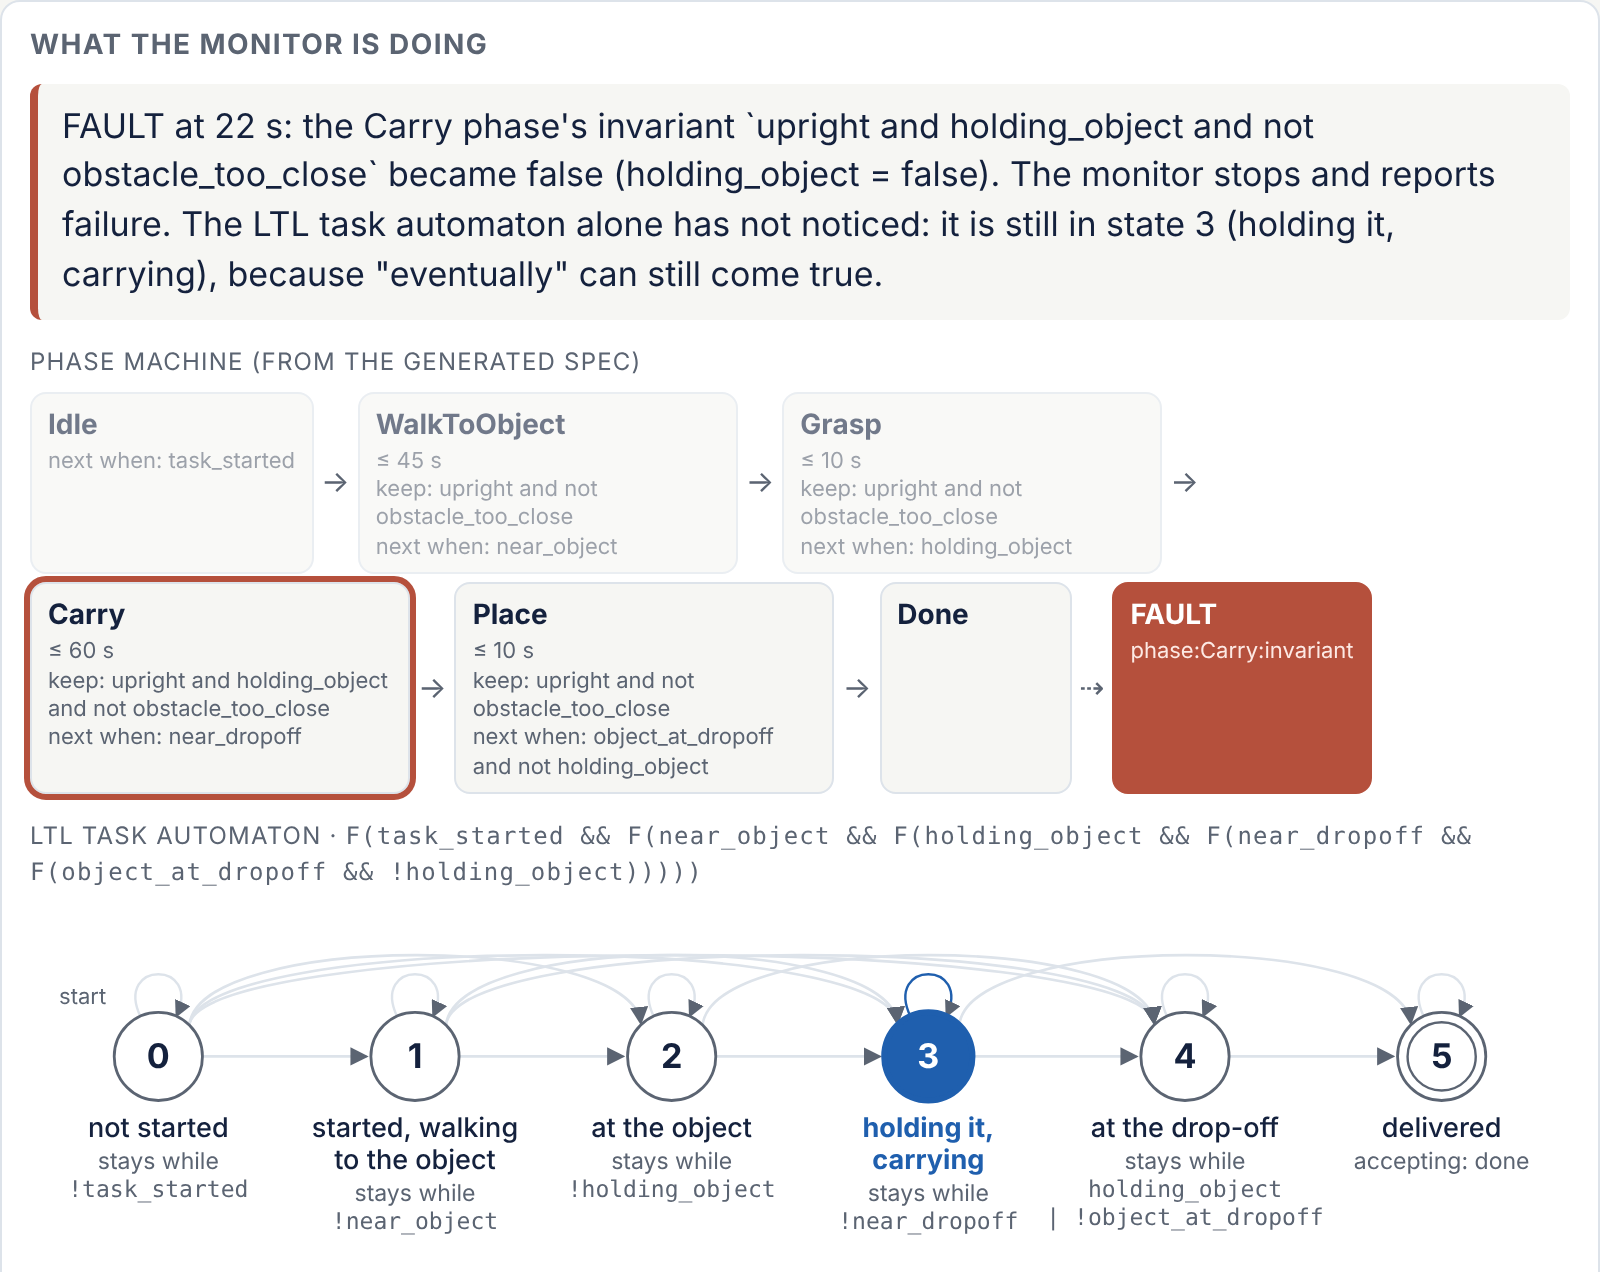
\includegraphics[width=\linewidth, height=0.66\textheight, keepaspectratio]{figures/automaton_card.png}
            \pic{From the live demo (one run). The current stage and state are lit.}
        \end{column}
    \end{columns}
\end{frame}

% --- DEADLINE ---
\begin{frame}{Does catching early matter?}
    \begin{columns}[c]
        \begin{column}{0.40\textwidth}
            \begin{itemize}
                \item With no time limit: all monitors $\approx$ 82--84\%.
                \item With a time limit: \key{64\%} with stages, 36\% without.
                \item Hand-written checks: 81\%, but someone must \textbf{predict every failure}.
            \end{itemize}
        \end{column}
        \begin{column}{0.58\textwidth}
            \centering
            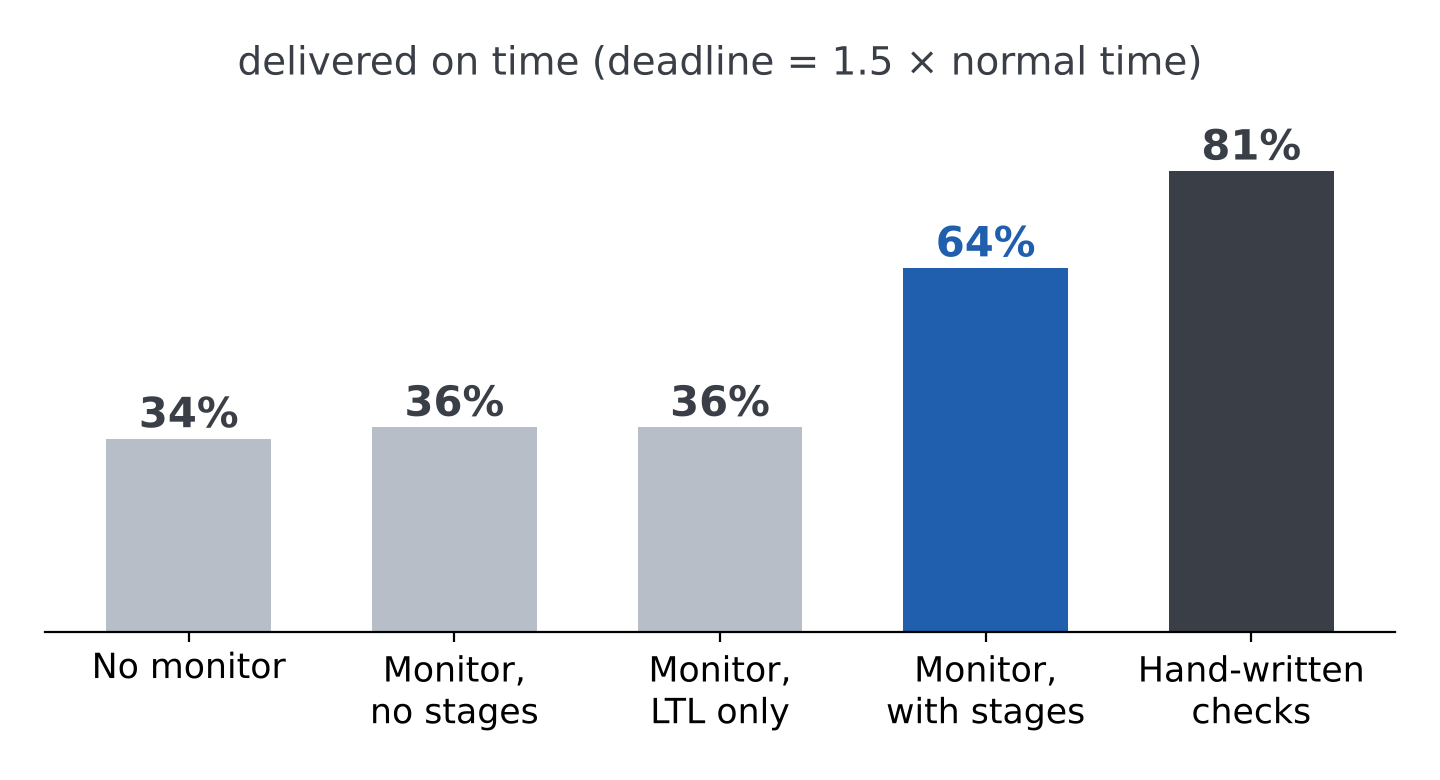
\includegraphics[width=\linewidth]{figures/chart_deadline.png}
            \pic{Tasks finished on time, 160 runs per bar. Early knowledge pays when time matters.}
        \end{column}
    \end{columns}
\end{frame}

% --- UNPLANNED FAILURES ---
\begin{frame}{Failures nobody planned for}
    \begin{columns}[c]
        \begin{column}{0.48\textwidth}
            \begin{itemize}
                \item Box left at the wrong place; robot too close to a wall.
                \item Hand-written checks: \textbf{\color{bad}40 of 40} missed.
                \item With our monitor: \key{0 of 40} missed.
                \item Missed by all: too slow, or a long detour.
            \end{itemize}
        \end{column}
        \begin{column}{0.50\textwidth}
            \centering
            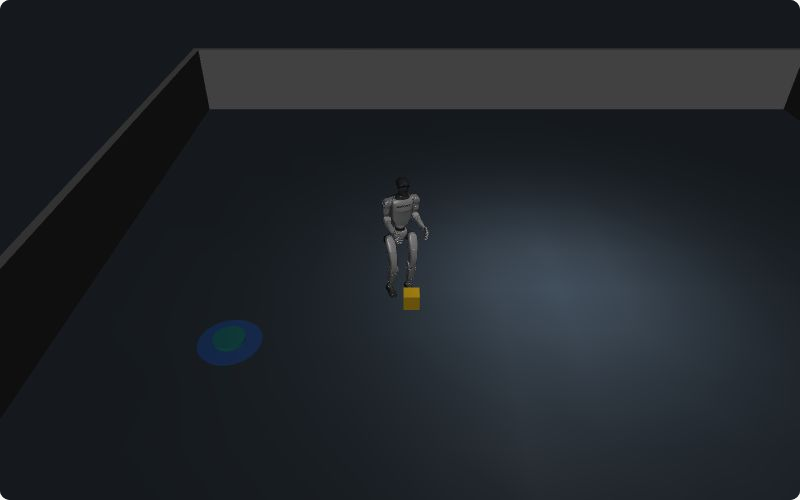
\includegraphics[width=\linewidth]{figures/robot_wrong_dropoff.png}
            \pic{The box is far from the drop-off (blue), yet the robot says ``done''. Our monitor catches it.}
        \end{column}
    \end{columns}
\end{frame}

% --- WHAT WE LEARNED ---
\begin{frame}{What we learned}
    \begin{columns}[c]
        \begin{column}{0.50\textwidth}
            \begin{itemize}
                \item \key{Stages catch failures when they happen.}
                \item Early alarms help \textbf{when time matters}.
                \item Rules come from words, so failures \textbf{nobody planned for} are caught too.
                \item Use the \textbf{robot's own sensors}, not the planner.
            \end{itemize}
        \end{column}
        \begin{column}{0.48\textwidth}
            \centering
            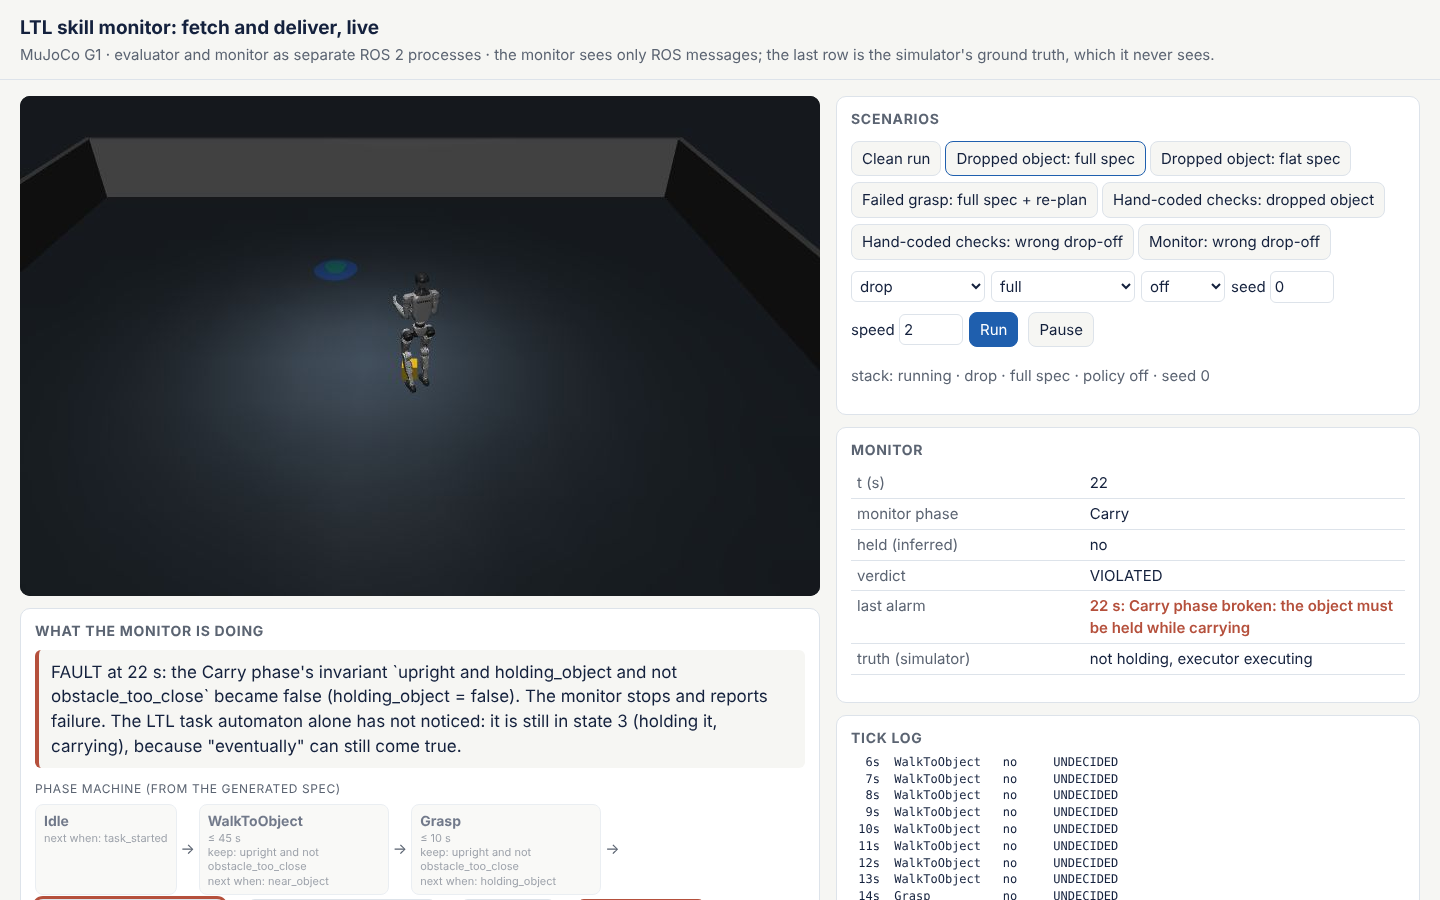
\includegraphics[width=\linewidth]{figures/demo_page.png}
            \pic{Live demo, one command:\\ \texttt{docker run -p 8080:8080 ghcr.io/pinhas019/ltlmonitor-demo}}
        \end{column}
    \end{columns}
\end{frame}

% --- TO BE DONE ---
\begin{frame}{To be done}
    \centering
    \resizebox{\linewidth}{!}{
    \begin{tikzpicture}[
        bx/.style={draw=mut, rounded corners=4pt, fill=soft, minimum height=3.4cm, text width=4.6cm, align=center},
        arr/.style={-{Stealth[length=2.5mm]}, thick, mut}]
        \node[bx, draw=acc, fill=acc!10] (a) {\textbf{1. Fix what we found}\\[0.2em] better time limits; progress toward each stage's own goal};
        \node[bx, right=0.5cm of a] (b) {\textbf{2. More tests}\\[0.2em] more tasks, more rule sets, more failures};
        \node[bx, right=0.5cm of b] (c) {\textbf{3. Real G1 robot}\\[0.2em] record, tune, monitor on vs.\ off};
        \node[bx, right=0.5cm of c] (d) {\textbf{4. The full POMDP}\\[0.2em] camera, real probabilities, best decisions};
        \draw[arr] (a) -- (b); \draw[arr] (b) -- (c); \draw[arr] (c) -- (d);
    \end{tikzpicture}
    }
    \vspace{0.3cm}

    \raggedright
    {\small \textbf{Limits today:} the grasp is simulated (no arms on this G1), the camera is simulated, the thresholds are not tuned.}
\end{frame}

% --- REFERENCES ---
\begin{frame}{References}
    \scriptsize
    \begin{itemize}
        \item[] Bauer, Leucker, Schallhart. \emph{Runtime Verification for LTL and TLTL.} ACM TOSEM 20, 2011.
        \item[] Chen, Gandhi, Zhang, Fan. \emph{NL2TL: Transforming Natural Languages to Temporal Logics using Large Language Models.} EMNLP 2023.
        \item[] Cosler, Hahn, Mendoza, et al. \emph{nl2spec: Interactively Translating Unstructured Natural Language to Temporal Logics with LLMs.} CAV 2023.
        \item[] Ferrando, Cardoso, Fisher, Ancona, et al. \emph{ROSMonitoring: A Runtime Verification Framework for ROS.} TAROS 2020.
        \item[] Kaelbling, Littman, Cassandra. \emph{Planning and Acting in Partially Observable Stochastic Domains.} Artificial Intelligence 101, 1998.
        \item[] Kapoor, Hammer, Kapoor, et al. \emph{Runtime Monitoring of Perception-Based Autonomous Systems via Embedding Temporal Logic.} arXiv:2605.12651, 2026.
        \item[] Lin, Duan, Fang, Fox, et al. \emph{FailSafe: Reasoning and Recovery from Failures in Vision-Language-Action Models.} arXiv:2510.01642, 2025.
        \item[] Liu, Yang, Idrees, Liang, et al. \emph{Grounding Complex Natural Language Commands for Temporal Tasks in Unseen Environments.} CoRL 2023.
        \item[] Stoller, Bartocci, Seyster, Grosu, Havelund, Smolka, Zadok. \emph{Runtime Verification with State Estimation.} RV 2011.
        \item[] Yamaguchi, Hoxha, Ni\v{c}kovi\'{c}. \emph{RTAMT: Runtime Robustness Monitors with Application to CPS and Robotics.} STTT 26, 2024.
        \item[] Zhang, Lu, Wang, Kang, et al. \emph{Foresight: Failure Detection for Long-Horizon Robotic Manipulation with Action-Conditioned World Model Latents.} arXiv:2606.23085, 2026.
    \end{itemize}
\end{frame}

\end{document}
